% mnras_template.tex
%
% LaTeX template for creating an MNRAS paper
%
% v3.0 released 14 May 2015
% (version numbers match those of mnras.cls)
%
% Copyright (C) Royal Astronomical Society 2015
% Authors:
% Keith T. Smith (Royal Astronomical Society)

% Change log
%
% v3.0 May 2015
%    Renamed to match the new package name
%    Version number matches mnras.cls
%    A few minor tweaks to wording
% v1.0 September 2013
%    Beta testing only - never publicly released
%    First version: a simple (ish) template for creating an MNRAS paper

%%%%%%%%%%%%%%%%%%%%%%%%%%%%%%%%%%%%%%%%%%%%%%%%%%
% Basic setup. Most papers should leave these options alone.

\documentclass[a4paper,fleqn,usenatbib]{mnras}

% MNRAS is set in Times font. If you don't have this installed (most LaTeX installations will be fine) or prefer the old Computer Modern fonts, comment out the following line

\usepackage{newtxtext,newtxmath}

% Depending on your LaTeX fonts installation, you might get better results with one of these:

%\usepackage{mathptmx}
%\usepackage{txfonts}

% Use vector fonts, so it zooms properly in on-screen viewing software. Don't change these lines unless you know what you are doing

\usepackage[T1]{fontenc}
\usepackage{ae,aecompl}

%%%%% AUTHORS - PLACE YOUR OWN PACKAGES HERE %%%%%

\usepackage{hyperref}
\usepackage[flushleft]{threeparttable}
\usepackage{pdflscape}

% Only include extra packages if you really need them. Common packages are:
\usepackage{graphicx}	% Including figure files
\usepackage{amsmath}	% Advanced maths commands
\usepackage{amssymb}	% Extra maths symbols

%%%%%%%%%%%%%%%%%%%%%%%%%%%%%%%%%%%%%%%%%%%%%%%%%%

%%%%% AUTHORS - PLACE YOUR OWN COMMANDS HERE %%%%%

\makeatletter
\newlength{\abovecaptionskip}%
\setlength{\abovecaptionskip}{10\p@}
\makeatother
\hypersetup{
    colorlinks=true,
    linkcolor=blue,
    filecolor=blue,      
    urlcolor=blue,
    citecolor=blue,
}
\newcommand{\fix}{\textcolor{red}}

% Please keep new commands to a minimum, and use \newcommand not \def to avoid
% overwriting existing commands. Example:
%\newcommand{\pcm}{\,cm$^{-2}$}	% per cm-squared

%%%%%%%%%%%%%%%%%%%%%%%%%%%%%%%%%%%%%%%%%%%%%%%%%%

%%%%%%%%%%%%%%%%%%% TITLE PAGE %%%%%%%%%%%%%%%%%%%

% Title of the paper, and the short title which is used in the headers. Keep the title short and informative.

\title[Escape Trajectories]{The Equilibrium Temperature of Planetary Bodies in Escape Trajectories}

% The list of authors, and the short list which is used in the headers. If you need two or more lines of authors, add an extra line using \newauthor

\author[M\'{e}ndez et al.]{
Abel M\'{e}ndez,$^{1}$\thanks{E-mail: abel.mendez@upr.edu}
Jorge Zuluaga,$^{2}$
Edgard Rivera-Valent\'{i}n,$^{3}$
Desiree Cotto-Figueroa$^{4}$
\\
% List of institutions
$^{1}$Planetary Habitability Laboratory, University 
of Puerto Rico at Arecibo, Arecibo, Puerto Rico\\
$^{2}$Institute of Physics / FCEN - Universidad de Antioquia, Antioquia, Colombia\\
$^{3}$Lunar and Planetary Institute \& Arecibo Observatory, USRA, Texas\\
$^{4}$Department of Physics and Electronics, University 
of Puerto Rico at Humacao, Humacao, Puerto Rico
}

% These dates will be filled out by the publisher
\date{Accepted XXX. Received YYY; in original form ZZZ}

% Enter the current year, for the copyright statements etc.
\pubyear{2018}

% Don't change these lines
\begin{document}
\label{firstpage}
\pagerange{\pageref{firstpage}--\pageref{lastpage}}
\maketitle

% Abstract of the paper

\begin{abstract}
Many comets, asteroids, and interstellar objects such as 1I/'Oumuamua move in escape trajectories and could experience large but transient variation in temperatures while passing a stellar system. These temperatures are usually calculated by numeric integration over a desired time period. Here we derived analytic solutions for the average equilibrium temperature of any planetary body in escape trajectories, including hyperbolic, parabolic, and linear paths. Our solutions were used to explore the net thermal effect of eccentricity and travel time. We found that 1I/'Oumuamua experienced a mild change in temperature compared to comets in similar trajectories and this probably contributed to the inactivity of any ices in its surface. Thus, interstellar objects in escape trajectories are less likely to exhibit cometary activity from orbital dynamics reasons alone even if ice rich.
\end{abstract}

% Select between one and six entries from the list of approved keywords. Don't make up new ones.

\begin{keywords}
radiation mechanisms: thermal -- methods: analytical -- comets: general -- minor planets, asteroids: individual (1I/2017 U1 'Oumuamua)
\end{keywords}

%%%%%%%%%%%%%%%%%%%%%%%%%%%%%%%%%%%%%%%%%%%%%%%%%%

%%%%%%%%%%%%%%%%% BODY OF PAPER %%%%%%%%%%%%%%%%%%

%% Section: Introduction
%%%%%%%%%%%%%%%%%%%%%%%%%%%%%%%%%%%%%%%%%%%%%%%%%%

\section{Introduction}

% About 1I/'Oumuamua

The interstellar asteroid 1I/'Oumuamua is the first known extrasolar visitor of our Solar System \citep{,2017MPEC....U..183M}. 1I/'Oumuamua was shown to describe a hyperbolic trajectory consistent with an extrasolar origin \citep{2017RNAAS...1....5D, 2017RNAAS...1...38W, 2017RNAAS...1...21M}. Its light curve suggests a tumbling elongated object (3-10:1 ratio) with an effective spherical radius of $102\pm4$ m and little to no cometary activity \citep{2017NatureMeech,2017ApJ...851L..31K,10.1038/s41550-018-0398-z}. The source and formation mechanism of 1I/'Oumuamua is still unknown but suggestions include an object ejected from a binary system, among many other alternatives \citep[\emph{e.g.},][]{2017RNAAS...1...13G, 2017RNAAS...1...18S, 2018ApJ...852L..13Z, 2018ApJ...852L..15C, 2017arXiv171103558P, 2017arXiv171106618D, 2017arXiv171107535F, 2017arXiv171109397Z, 2017arXiv171108800F, 2018arXiv180102821D}.

% About equilibrium temperature and escape orbits

The average equilibrium temperature of a planetary body helps to define its general thermal state between the extreme temperatures near periastron and apastron \citep{2017ApJ...837L...1M}. Bodies in escape trajectories could experience dramatic thermal variations, from the long interstellar environment to transient but strong stellar fluxes at periastron. This is true for 1I/'Oumuamua and many known comets and asteroids with parabolic and near hyperbolic trajectories in the Solar System \citep{SSD(2018)}. Other planetary bodies in highly eccentric elliptical orbits experience similar but periodic wide thermal variations (\emph{e.g.} comet 1P/Halley).

% About surface temperature of airless bodies

The surface temperature of small planetary bodies plays a key role in assessing their ice loss rates \citep{2018arXiv180201293S}. In equilibrium, it is similar to the interior temperature and depends, beside orbital factors, on the albedo, thermal inertia, and the spin axis tilt of the body. The average surface temperature is about 1\% lower than the equilibrium temperature for a fast rotator with a zero axis tilt and high thermal inertia, and given by
\begin{equation} \label{eq:Ts}
\langle T_s \rangle = \frac{\pi^{1/4}}{5\sqrt{2}} \frac{\Gamma(1/8)}{\Gamma(5/8)} \, \langle T_{eq} \rangle \approx 0.98882 \, \langle T_{eq} \rangle
\end{equation}
where $\langle T_s \rangle$ and $\langle T_{eq} \rangle$ are the global- and time-averaged surface and equilibriun temperatures, respectively \citep{2018arXiv180201293S}. If the only energy source is from isolation, then it is
always the case that $\langle T_s \rangle$ < $\langle T_{eq} \rangle$. For dust covered bodies (\emph{i.e.}, low thermal conductivity), the surface temperature
can easily be 20 K lower, which drastically reduces sublimation rates \citep{2008ApJ...682..697S, 2016Icar..276...88S}.

% About surface temperature and ice loss

The rapid change of surface temperatures over a moderately short-time period might produce outgassing of ices in planetary bodies, especially comets. For example, ESA's Rosetta mission monitored a set of eight molecules, including CH$_4$, NH$_3$, H$_2$O, HCN, CO, O$_2$, H$_2$S and CO$_2$, for several weeks post-perihelion, from 2.0 to 3.5 AU, of comet 67P/Churyumov-Gerasimenko \citep{2017MNRAS.469S.108G}. These observations provided an unique opportunity to compare not only the different outgassing patterns of these molecules in a comet, but also their temporal variations as function of illumination. The total outgassing was always dominated by water in the pre-perihelion period \citep{2016MNRAS.462S.156F}. Water seems to follow the sub-solar latitude, which was expected given its rather high sublimation temperature \citep{2016MNRAS.462S.491H}. The general decrease over the period in molecular abundances varies greatly from molecule and it does not follow the sublimation temperatures of pure ices (Table \ref{tab:ices}).

% Table: Ice Sublimation Temperatures

\begin{table}
\centering
\begin{threeparttable}
\centering
\caption{Representative abundances of ices in comets and their sublimation temperatures $T_{sub}$ in vacuum conditions.}
\begin{tabular}{ c c c }
 \hline
 \hline
	Molecule & Abundance (\%)\tnote{a} & $T_{sub}$ (K)\tnote{b} \\
 \hline
	H$_2$O & 100 & 144 \\
	CO$_2$ & 2 - 30 & 86 \\
	CO & 0.4 - 30 & 28 \\
	CH$_4$ & 0.4 - 1.6 & 36 \\
	NH$_3$ & 0.2 - 1.4 & 102 \\
	H$_2$S & 0.12 - 1.4 & 80 \\
	HCN & 0.1 - 0.25 & 126 \\
	O$_2$ & - & 30 \\
 \hline
 \hline
\end{tabular}
\label{tab:ices}
	\begin{tablenotes}
	\small
\item[a]{Abundances relative to water from Table 3 and 4 of \citet{2011ARA&A..49..471M}.}
\item[b]{Sublimation temperatures from Table 2 of \citet{2017MNRAS.469S.108G}.}
	\end{tablenotes}
\end{threeparttable}
\end{table}

% About bond albedo

One of the most important planetary properties to calculate the equilbrium temperature is the bolometric albedo $A$, also known as the Bond albedo albeit with conflicting definitions in the literature \citep{1916PNAS....2...74R, 1981A&A...104...42H, 1999PCEC...24..573G,2016AJ....152..209M}. The bolometric and geometric albedos are related by $A = qA_g$ where $A_g$ is the geometric albedo and $q$ is the phase integral. The bolometric is the albedo as derived by accounting for the full scattering of the surface over all phase angles and wavelengths, while the geometric is the albedo at zero phase angle (\emph{i.e.}, viewing the object directly at opposition along the site of illumination), and can be a function of wavelength. As such, $A$ is always between zero and one and $A_g$ can be higher than one, depending on the scattering properties normalized to an ideal surface (\emph{e.g.} for Enceladus $A=0.8$ and $A_g=1.4$).

% About spherical bond albedo

Because $A$ requires more information to calculate a significant $q$, it is not easy to relate to $A_g$. For example, the spherical albedo $A_s$ for an ideal Lambertian surface at a specific wavelength is related to the geometric albedo by $A_s=\frac{3}{2}A_g$, but this assumption overestimates $A$ \citep{2016ApJ...822...76D}. When possible, the $A$ should be calculate as a function of latitude and longitude for a given shape model because it also dependent on the scattering properties and topography of the body. Alternatively, a spherical bolometric albedo can be calculated as a gross body wide value. For asteroids and comets this is a rough approximation because it assumes a spherical shape, and they are rarely spheres.

% About bond albedo estimates for asteroids

Nevertheless, it is possible to estimate approximate spherical bolometric albedos for asteroids from their visual geometric albedos using the empirical relation
\begin{equation} \label{eq:albedo}
A=(0.290+0.684G)A_g
\end{equation}
where the slope parameter $G$ describes the change in the brightness of the object at different illumination phase angles \citep{2008Icar..195..674S}. A mean value of $G = 0.18 \pm 0.13$ could be used for asteroids based on observational data from the JPL Small-Bodies Database \citep{2013PhDT.......424C}. Thus, the average bolometric albedos for asteroids can be estimated from equation \ref{eq:albedo} and their distribution of geometric albedos (Table \ref{tab:asteroids}). \citet{2013ApJ...762...56U} calculated geometric albedos for 5120 asteroids measured by the infrared astronomical satellite AKARI. See for example \citet{1989aste.conf..524B}, \citet{2011LPI....42.1028S}, \citet{2013Icar..226.1252L} or \citet{2015aste.book..107D} for more details on the calculation of bolometric albedos of asteroids from photometric data.  

% Table: Asteroids

\begin{table*}
\begin{threeparttable}
\centering
\caption{General properties of S, X, and C type asteroids.\tnote{a}}
\begin{tabular}{ c c c c }
 \hline
 \hline
Spectral Type & Abundance (\%) & Density (gcm$^{-3}$) & $A_g$ \\
\hline
	S & 62 & 2.660 $\pm$ 0.594 & 0.26 $\pm$ 0.035 \\
	X & 22 & 2.819 $\pm$ 0.631 & 0.31 $\pm$ 0.075 \\
	C & 16 & 1.626 $\pm$ 0.568 & 0.13 $\pm$ 0.055 \\
 \hline
 \hline
\end{tabular}
\label{tab:asteroids}
	\begin{tablenotes}
	\small
\item[a]{Adapted from \citet{2013PhDT.......424C}.}
	\end{tablenotes}
\end{threeparttable}
\end{table*}

% About the goal of this study

The goal of our study is to compare the thermal state between planetary bodies in closed and open trajectories. We derive analytic solutions for the temporal average of orbital distance, stellar flux, and equilibrium temperature of planetary bodies in escape trajectories. They where derived by integration with respect to time as described in \citet{2017ApJ...837L...1M} for elliptical orbits. Our solutions were also compared with circular and elliptical orbits as defined in Table \ref{tab:summary} and shown in Figure \ref{fig1}. 

% About the content of this paper

Section \ref{sec:elliptical} describes solutions of elliptical orbits for comparison purposes. Sections \ref{sec:parabolic}, \ref{sec:hyperbolic}, and \ref{sec:linear} present our new derivations for parabolic, hyperbolic, and linear trajectories, respectively. Section \ref{sec:discussion} discuss the validation of our results with numerical simulations and applications to Solar System and extrasolar planetary bodies, including I1/'Oumuamua.

% Figure: Orbits comparison

\begin{figure}
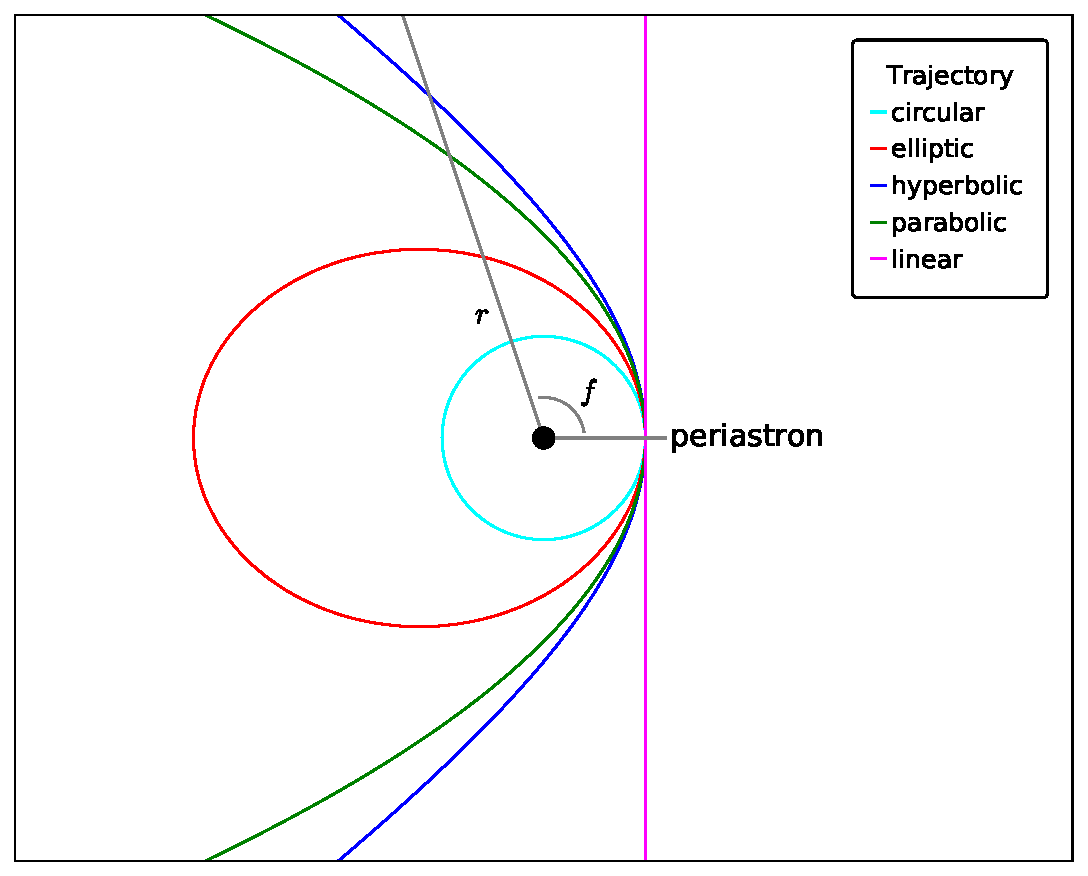
\includegraphics[width=\columnwidth]{f1.pdf}
\caption{Comparison of escape trajectories with those of circular and elliptical orbits with a common periastron.}
\label{fig1}
\end{figure}

%% Section: Elliptical Orbits
%%%%%%%%%%%%%%%%%%%%%%%%%%%%%%%%%%%%%%%%%%%%%%%%%%

\section{Elliptical Orbits} \label{sec:elliptical}

% About previous work on elliptic orbits

Temporal averages for orbital distance $\langle r \rangle$, stellar flux $\langle F \rangle$, and equilibrium temperature $\langle T_{eq} \rangle$ for elliptic orbits were derived by \citet{2017ApJ...837L...1M}. They were solved by calculating the average value integrating over time $t$ around the orbital period $T$ and making the substitutions $r=a(1-e\cos{E})$, $M=E-e\sin{E}$, and $M=(2\pi/T)t$; where $r$ is position, $e$ is the orbital eccentricity, $a$ is the semi-major axis in astronomical units, $E$ is the eccentric anomaly, and $M$ is the mean anomaly. These averages are
% elliptic equations
\begin{equation} \label{eq:re}
\langle r \rangle = a\left ( 1+\frac{e^2}{2} \right ),
\end{equation}
\begin{equation} \label{eq:Fe}
\langle F \rangle = \frac{L}{a^2\sqrt{1-e^2}},
\end{equation}
\begin{equation} \label{eq:Te}
\langle T_{eq} \rangle = T_o\left[ \frac{(1-A)L}{\beta \epsilon a^2}\right] ^\frac{1}{4}\frac{2\sqrt{1+e}}{\pi} \; \mathbf{E}\left ( \frac{2e}{1+e} \right ),
\end{equation}
where $L$ is the stellar luminosity in solar units, $A$ the bond albedo, $\epsilon$ the emissivity, $\beta$ the redistribution factor, $T_o$ = 278.5 K, and $\mathbf{E}$ is the complete elliptic integral of the second kind \citep{MathWorld, GSL}. The definition of $\mathbf{E}(2e/(1+e))$ used in equation \ref{eq:Te} is the one implemented in software packages like \emph{Mathematica} (\emph{i.e.}, \texttt{EllipticE}) and \emph{Maxima} (\emph{i.e.}, \texttt{elliptic$\_$ce}). The \emph{GNU Scientific Library} (GSL) uses \texttt{gsl\_sf\_ellint\_Ecomp} which requires first the square root of the argument (\emph{i.e.}, $\mathbf{E}(\sqrt{2e/(1+e)}$).

% About previous work conclusion

For elliptical orbits the average distance ($a \leq \langle r \rangle < \frac{3}{2}a$) and stellar flux ($F|_{e=0} \leq \langle F \rangle < \infty$) increase with eccentricity. However, the average equilibrium temperature ($T_{eq}|_{e=0} \leq \langle T_{eq} \rangle < \frac{2\sqrt{2}}{\pi} T_{eq}|_{e=0}$) slowly decreases with eccentricity until converging to $\sim90\%$ of the equilibrium temperature for circular orbits (Figure  \ref{fig2}). Table \ref{tab:elliptic} shows these averages calculated for some minor planetary bodies with highly eccentric orbits. Note that the $\langle T_{eq} \rangle$ of comet 1P/Halley is about 70 K and not 92 K from the commonly assumed but incorrect expression $\langle T_{eq} \rangle = T_o [\langle F \rangle(1-A)]^\frac{1}{4}$.

% About new equations for elliptical orbits

Equations \ref{eq:re} to \ref{eq:Te} are averages for a full orbital period, but to compare with escape trajectories we also derived expressions for the path near periastron $E=0$ between the eccentric anomalies $-E_o$ to $+E_o$. From the integration over time we obtained
% elliptic equations (arc)
\begin{equation} \label{eq:re2}
\langle r \rangle = a \left[ \frac{{{\left(e^{2} + 2\right)} E_o} + {e\left(e \cos{E_o} - 4\right)} \sin{E_o}}{2 \, {\left(E_o - e\sin{E_o}\right)}} \right],
\end{equation}
\begin{equation} \label{eq:Fe2}
\langle F \rangle = \frac{L}{a^2} \left[ \frac{2 \tan^{-1}\left(\sqrt{\frac{1 + e}{1 - e}} \tan{\frac{1}{2} E_o}\right)}{ {\left(E_o - e \sin{E_o} \right)}\sqrt{1-e^{2}}} \right],
\end{equation}
\begin{multline} \label{eq:Te2}
\langle T_{eq} \rangle = T_o \left[\frac{L {\left(1-A\right)}}{a^{2}}\right]^{\frac{1}{4}} \frac{2 i \,  \sqrt{1-e}}{ E_o - e \sin{E_o} } \ldots \\
\left(\mathbf{E} \left(q \,\big|\,p \right) - \mathbf{F} \left(q \,\big|\,p\right) -i \, \sqrt{\frac{1- e \cos{E_o}}{1 - e}} \tan{\frac{1}{2} E_o} \right)
\end{multline}
where $q = i \, \sinh^{-1}(\tan{\frac{1}{2} E_o})$, $p=(1+e)/(1-e)$, $\mathbf{E}$ is the incomplete elliptic integral of the second kind, and $\mathbf{F}$ is the incomplete elliptic integral of the first kind.

% Figure: Comparison of averages for elliptic orbits

\begin{figure}
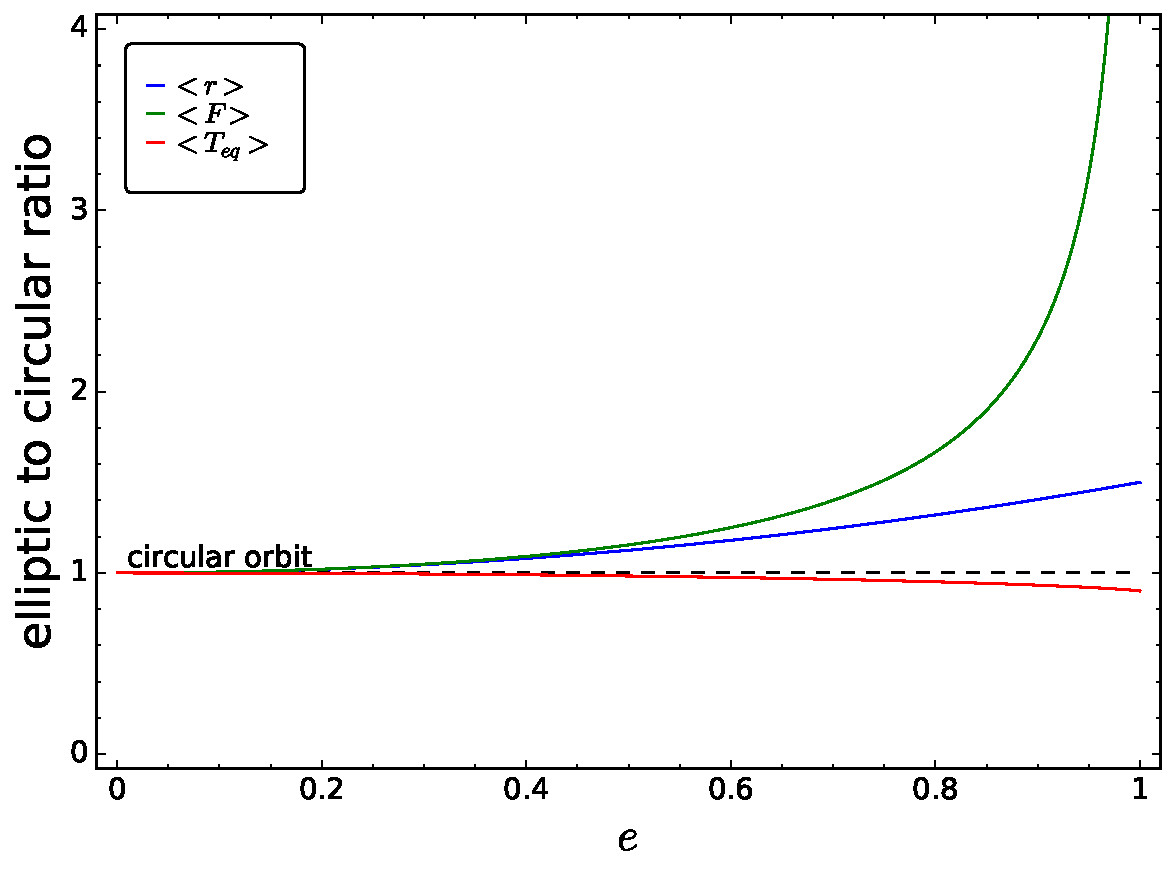
\includegraphics[width=\columnwidth]{f2.pdf}
\caption{Comparison of temporal averages of orbital distance, stellar flux, and equilibrium temperature as a function of eccentricity $e$ for elliptical orbits with constant semi-major axis (normalized with respect to circular orbits).}
\label{fig2}
\end{figure}

% Table: Sample objects in elliptic orbits

\begin{table*}
\begin{threeparttable}
\centering
\caption{Temporal averages of orbital distance $\langle r \rangle$, stellar flux $\langle F \rangle$, and equilibrium temperature $\langle T_{eq} \rangle$ for some  planetary bodies with eccentric orbits ($e$ > 0.2) including comets, asteroids, Trans-Neptunian Objects (TNO), and planets.}
\begin{tabular}{ l c c c c c c c c }
 \hline
 \hline
 & \multicolumn{5}{c}{Object Description\tnote{a}} & \multicolumn{3}{c}{Temporal Averages\tnote{d}} \\
 \hline
 Name & Type & $a$ (AU) & $e$ & $A_g$\tnote{b} & $A$\tnote{c} & $\langle r \rangle$ (AU) & $\langle F \rangle$ & $\langle T_{eq} \rangle$ (K) \\ 
 \hline
 1P/Halley & HTC & 17.834145 & 0.96714291 & 0.04 & 0.02 & 26.174  & 0.0123 & 60.0 \\  
 2P/Encke & JFC & 2.2151323 & 0.84832024 & 0.046 & 0.02 & 3.0122 & 0.384 & 176 \\
 9P/Tempel 1 & JFC & 3.1457942 & 0.50964598 & 0.056 & 0.013 & 3.5543 & 0.117 & 154 \\
 67P/Churyumov-Gerasimenko & JFC & 3.4647374 & 0.64058232 & 0.06 & 0.03 & 4.1756  & 0.108 & 144 \\
 81P/Wild 2 & JFC & 3.4518811 & 0.53707199 & 0.063 & 0.012 & 3.9497 & 0.0994 & 147 \\ 
 103P/Hartley 2 & JFC & 3.4725219 & 0.69512663 & 0.045 & 0.012 & 4.3114 & 0.115 & 144 \\
 253 Mathilde & C & 2.6506802 & 0.26320066 & 0.041 & 0.013 & 2.7424 & 0.148 & 170 \\
 433 Eros & S & 1.45794 & 0.22258897 & 0.23 & 0.092 & 1.4941 & 0.483 & 224 \\
 1566 Icarus & S & 1.0779459 & 0.8268093 & 0.29 & 0.08 & 1.4464  & 1.53 & 249 \\
 9969 Braille & Q & 2.3410243 & 0.43344223 & 0.34 & 0.14 & 2.5609 & 0.204 & 173 \\
 25143 Itokawa & S & 1.3241134 & 0.28016847 & 0.33 & 0.14 & 1.3760 & 0.594 & 232 \\
 101955	Bennu & B & 1.126391 & 0.20374511 & 0.047 & 0.016   & 1.1498 & 0.805 & 261 \\
 90377 Sedna & SD? & 487.7651 & 0.8440912 & 0.32 & 0.19 & 661.53  & $7.84\times10^{-6}$ & 11.3 \\
 90482 Orcus & KBO & 39.3976243 & 0.22008902 & 0.28 & 0.15 & 40.352 & $6.60\times10^{-4}$ & 42.5 \\
 134340 Pluto & KBO & 39.4450697 & 0.25024871 & 0.62 & 0.72 & 40.680 & $6.64\times10^{-4}$ & 32.1 \\
 136199 Eris & SD & 67.6487798 & 0.44172397 & 0.96 & 0.55 & 74.249 & $2.44\times10^{-4}$ & 27.4 \\
 225088	2007 OR$_{10}$ & SD & 67.1436607 & 0.50577423 & 0.089 & 0.06 & 75.731 & $2.57\times10^{-4}$ & 32.9 \\
 Mercury & Planet & 0.38709927 & 0.20563593 & 0.106 & 0.088 & 0.3953 & 6.82 & 436 \\
 \hline
 \hline
\end{tabular}
\label{tab:elliptic}
	\begin{tablenotes}
	\small
\item[a]{Object elements from the NASA Solar System Dynamic website \href{https://ssd.jpl.nasa.gov/?sb$\_$elem}{https://ssd.jpl.nasa.gov/?sb$\_$elem}.}
\item[b] {Geometric albedos from \citet{2004come.book..223L,2010AJ....139.2700B,2011Natur.478..493S,2012A&A...541L...6P,2015ApJ...814..117N,2015Sci...347a0628C,2015Icar..252..393T,2016AJ....151..117P}, and Table 6 of \citet{2013Icar..226.1252L}.}
\item[c] {Bond albedos from \citet{1981motc.conf...83C,1987Icar...69...33H,2004Icar..167..129B,2010AJ....139.2700B,2011Natur.478..493S,2015Icar..252..393T,2017arXiv170302670M,2017Icar..287..207B}, Table 6 of \citet{2013Icar..226.1252L}, and Table 1 of \citet{2015ApJ...809...43J}. Value for 1566 Icarus assuming the average for S-type asteroids. Value for 90482 Orcus assuming a phase integral of $q$ $\approx$ 0.55, similar to the icy satellites of Uranus.}
\item[d]{Average values calculated with equations \ref{eq:re}, \ref{eq:Fe}, and \ref{eq:Te}, respectively. Equilibrium temperatures assuming a fast rotator ($\beta$=1) with unit emissivity ($\epsilon$=1).}
	\end{tablenotes}
\end{threeparttable}
\end{table*}

%% Section: Parabolic Trajectories
%%%%%%%%%%%%%%%%%%%%%%%%%%%%%%%%%%%%%%%%%%%%%%%%%%

\section{Parabolic Trajectories}
\label{sec:parabolic}

% About calculations for parabolic trajectories

Planetary bodies with speeds near the escape velocity around a star move in parabolic paths. We integrated the averages for parabolic trajectories taking $r=r_p(1+D^2)$, $M=D+\frac{1}{3}D^3$, and $M=(2M_o/T)t-Mo$; where $D$ is the parabolic anomaly from $-D_o$ to $+D_o$. They are given by
% parabolic equations
\begin{equation} \label{eq:rp}
\langle r \rangle = r_p \left[ \frac{3 {D_o}^{4} + 10 {D_o}^{2} + 15}{5 \left({D_o}^{2} + 3\right)} \right],
\end{equation}
\begin{equation} \label{eq:Fp}
\langle F \rangle = \frac{L}{r_p^2} \left[ \frac{3 \tan^{-1} D_o}{{\left({D_o}^2 + 3\right)} D_o} \right],
\end{equation}
\begin{equation} \label{eq:Tp}
\langle T_{eq} \rangle = T_o \left[\frac{L {\left(1 - A\right)}}{\beta \epsilon r_p^{2}}\right]^{\frac{1}{4}} \left[ \frac{3 {\left(D_o\sqrt{{D_o}^{2} + 1} + \sinh^{-1} D_o \right)}}{2 \, {\left({D_o}^{2} + 3\right)} D_o} \right].
\end{equation}

% About trends in parabolic orbits

The average distance ($r_p \leq \langle r \rangle < \infty$) increase with orbital time (\emph{i.e.} large $D_o$) to infinity as expected for open orbits such as a parabolic trajectories. Accordingly, the average stellar flux ($F(r_p) \leq \langle F \rangle < 0$) and equilibrium temperature ($T_{eq}(r_p) \leq \langle T_{eq} \rangle < 0$) decreases with time to zero.

%% Section: Hyperbolic Trajectories
%%%%%%%%%%%%%%%%%%%%%%%%%%%%%%%%%%%%%%%%%%%%%%%%%%

\section{Hyperbolic Trajectories}
\label{sec:hyperbolic}

% About calculations for hyperbolic trajectories

Planetary bodies with speeds over the escape velocity around a star move in hyperbolic paths. The period of integration $T$ was taken from entering to leaving the stellar system where the time to periastron is the semi-period $\frac{1}{2}T$. The integrals were solved by making the substitutions $r=r_p(1-e\cosh{H})/(1-e)$, $M=e\sinh{H} - H$, and $M=(2M_o/T)t - M_o$; where $r_p$ is the periastron, $H$ is the hyperbolic eccentricity and the objects move between time zero to $T$, corresponding to $-M_o$ to $+M_o$ in the mean anomaly and $-H_o$ to $+H_o$ in the hyperbolic anomaly. The distance, stellar flux, and equilibrium temperature averages are then given with respect to the hyperbolic anomaly as
% hyperbolic equations
\begin{equation} \label{eq:rh}
\langle r \rangle = r_p \left[\frac{e \left(e \cosh{H_o} - 4\right) \sinh{H_o} + \left(e^{2} + 2\right) H_o}{2\left(e \sinh{H_o} - H_o\right) \left( e-1 \right) } \right],
\end{equation}
\begin{equation} \label{eq:Fh}
\langle F \rangle = \frac{L}{r_p^2} \left[ \frac{2 \left( e - 1 \right)^2 \left(e^2 - 1\right)^{-\frac{1}{2}}}{e \sinh{H_o} - H_o}\tan^{-1}\left({\frac{\left(e + 1\right) \tanh{\frac{1}{2}H_o}}{\sqrt{e^2 - 1}}}\right) \right],
\end{equation}
\begin{equation} \label{eq:Th}
\langle T_{eq} \rangle = T_o \left[\frac{L {\left(1 - A\right)}}{\beta \epsilon r_p^{2}}\right]^{\frac{1}{4}} \left[ \frac{-2 i \left(e-1\right)}{e \sinh{H_o} - H_o} \, {\rm \mathbf{E}}\left(\tfrac{1}{2}iH_o \, \big| \, \frac{2e}{e - 1}\right) \right]
\end{equation}
where $\mathbf{E}$ is the incomplete elliptic integral of the second kind \citep{MathWorld, GSL}. As in equation \ref{eq:Te}, the definition of $\mathbf{E}$ used in equation \ref{eq:Th} is the one implemented in \emph{Mathematica} or \emph{Maxima} and not in GSL. Note that equation \ref{eq:Th} also involves operations with imaginary numbers.

% About trends in hyperbolic orbits

For hyperbolic trajectories the average distance ($r_p \leq \langle r \rangle < \infty$) increase with orbital time (\emph{i.e.} large $H_o$) to infinity, but decreases with eccentricity. The average stellar flux ($F(r_p) \leq \langle F \rangle < 0$) and equilibrium temperature ($T_{eq}(r_p) \leq \langle T_{eq} \rangle < 0$) decreases with time to zero, but the flux decreases with eccentricity while the temperature increases. All these averages converge to those of a linear trajectory (Section \ref{sec:linear}) for large eccentricities (Figure \ref{fig3}).

% Figure: Comparison of averages for hyperbolic orbits

\begin{figure}
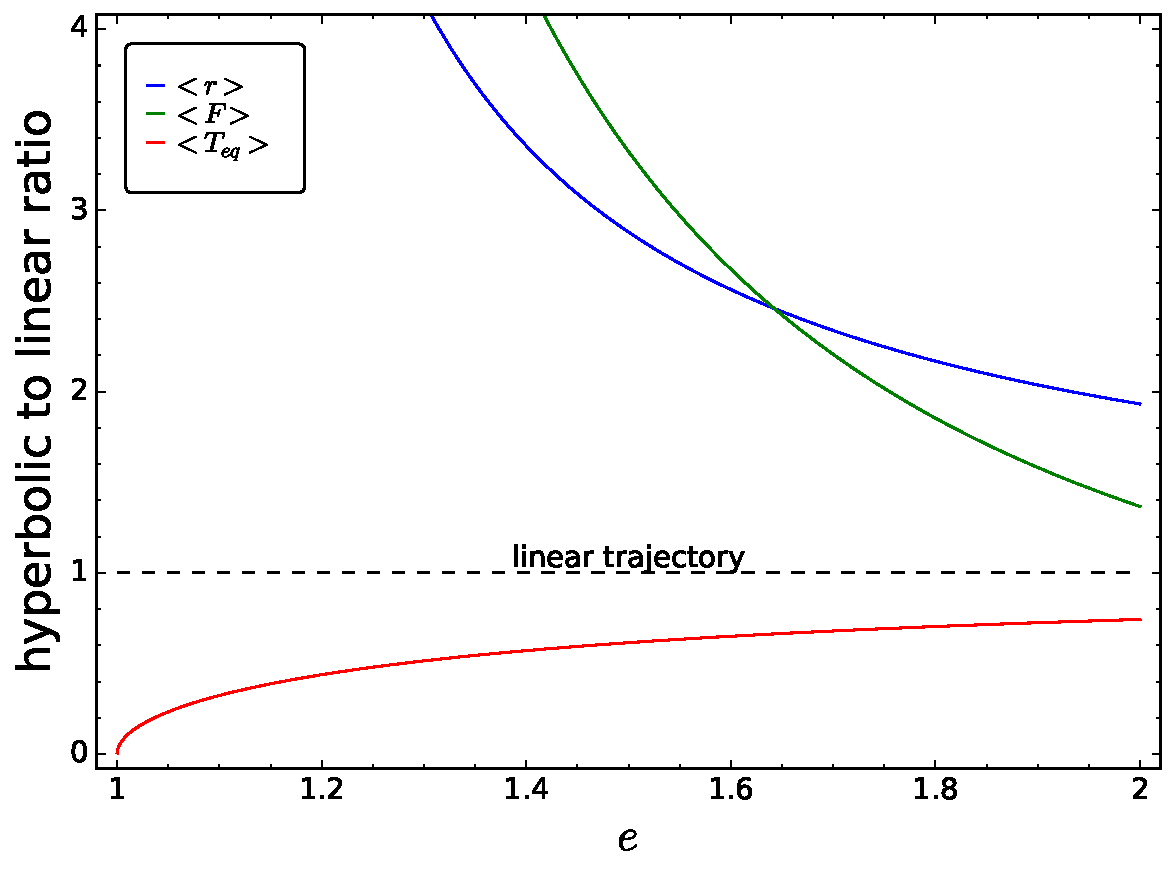
\includegraphics[width=\columnwidth]{f3.pdf}
\caption{Comparison of temporal averages of orbital distance, stellar flux, and equilibrium temperature as a function of eccentricity $e$ for hyperbolic trajectories with constant periastron (normalized with respect to linear trajectories). Hyperbolic trajectories converge to linear trajectories for $e \to \infty$.}
\label{fig3}
\end{figure}

%% Section: Linear Trajectories
%%%%%%%%%%%%%%%%%%%%%%%%%%%%%%%%%%%%%%%%%%%%%%%%%%

\section{Linear Trajectories}
\label{sec:linear}

% About calculations for linear trajectories

Planetary bodies that are moving fast and far from a star  could move in near-linear paths. These trajectories are a special case of the hyperbolic trajectories where $e$ equal to infinity. We solved equations \ref{eq:rh} to \ref{eq:Th} for $\lim\limits_{e \to \infty}$ obtaining
% linear equations
\begin{equation} \label{eq:rl}
\langle r \rangle = r_p \left[\frac{\sinh 2H_o  + 2H_o}{4 \sinh H_o } \right],
\end{equation}
\begin{equation} \label{eq:Fl}
\langle F \rangle = \frac{L}{r_p^2} \left[ \frac{2 \tan^{-1} \left( \tanh \frac{1}{2} H_o \right)}{\sinh H_o } \right],
\end{equation}
\begin{equation} \label{eq:Tl}
\langle T_{eq} \rangle = T_o \left[\frac{L {\left(1 - A\right)}}{\beta \epsilon r_p^{2}}\right]^{\frac{1}{4}} \left[ \frac{-2 i}{\sinh H_o } {\rm \mathbf{E}} \left(\tfrac{1}{2}iH_o\, \big| \,2 \right) \right].
\end{equation}

% About trends in linear trajectories

For linear trajectories the average distance ($r_p \leq \langle r \rangle < \infty$) increase with orbital time (\emph{i.e.} large $H_o$) to infinity. The average stellar flux ($F(r_p) \leq \langle F \rangle < 0$) and equilibrium temperature ($T_{eq}(r_p) \leq \langle T_{eq} \rangle < 0$) decreases with time to zero.

%% Discussion
%%%%%%%%%%%%%%%%%%%%%%%%%%%%%%%%%%%%%%%%%%%%%%%%%%

\section{Discussion}
\label{sec:discussion}

% About validation with numerical integration

Our analytic solutions for the average distance, stellar flux, and equilibrium temperature of planetary bodies in elliptic, parabolic, hyperbolic, and linear trajectories (Equations \ref{eq:re} to \ref{eq:Tl}) were validated with numerical solutions. We performed numerical integrations of the average function with respect to time in IDL using the fourth-order Runge-Kutta procedure \texttt{RK4}. Both the analytic expressions and numerical solutions agreed in all cases. We also verified our solutions with a boundary-value analysis with respect to eccentricity and conic anomalies (\emph{i.e.}, the elliptical, parabolic, and hyperbolic anomalies). The perihelion elliptic solutions (equations \ref{eq:re2} to \ref{eq:Te2}) converge to the full orbit elliptic solutions (equations \ref{eq:re} to \ref{eq:Te}) for $E_o = \pi$. The hyperbolic solutions (equations \ref{eq:rh} to \ref{eq:Th}) converge to the linear solutions (equations \ref{eq:rl} to \ref{eq:Tl}) for $e \rightarrow \infty$.

% About Limitations

Our solutions assume that the albedo remains constant during the trajectory. This might be true for airless bodies such as asteroids but not necessarily for comets, especially near perihelion and after the formation of the coma. For instance, dust from the coma might increase the total sunlight reaching the nucleus. The coma provides an isotropic source of scattered sunlight and thermal emission over the entire nucleus surface due to its significantly greater geometrical cross section as compared with the nucleus \citep{1981Icar...47..302W}. Also, significant mass losses could expose materials with different ice/dirt ratios and hence different thermal or optical properties \citep{1984Icar...57...55H}. All these processes are a strong function of heliocentric distance and more significant for near-Sun comets (\emph{i.e.}, $r_p$ < 0.307 AU) \citep{2018SSRv..214...20J}. However, we are assuming here that heliocentric variations in the bolometric albedo are negligible for simplicity.

% About how to define the limits for averages

The averages for escape trajectories become $\left<r\right>=\infty$, $\left<F\right>=0$, and $\left<T_{eq}\right>=0$ for large times. Thus, they are meaningless unless they are calculated with respect to some fixed boundaries. One alternative is to calculate these averages after some heliocentric distance when the planetary body is considered under the influence of the Solar System (\emph{e.g.} within the heliopause $\sim122$ AU, \citet{2017ApJ...834..197C}). Other alternative is to use some standard time of comparison around periastron (\emph{e.g.} one year). Another alternative is to calculate averages after the body is above some critical temperature (\emph{e.g.} 170 K snow line, \citet{2008ApJ...673..502K}).

% About Comparing hyperbolic and elliptic trajectories

One way to compare hyperbolic trajectories with elliptic orbits is under the same time frame. This could be the orbital period of the elliptic orbit but with the same periastron of the hyperbolic trajectory (periods shown in Table \ref{tab:summary}). We calculated the ratio between the average equilibrium temperature of hyperbolic trajectories $\left<T_{eq}\right>_H$ and that of elliptic orbits $\left<T_{eq}\right>_E$ for the same periastron and period (Figure \ref{fig4}). The temperatures for hyperbolic orbits are always less than that of the equivalent elliptic orbits for any combination of the elliptic and hyperbolic eccentricities. Temperatures also decrease with the hyperbolic eccentricity. This trend is also true for parabolic and linear trajectories. Therefore, planetary objects in escape trajectories always experience lower temperatures than those in equivalent elliptical orbits (\emph{i.e.} same period and periastron).

% Figure: Comparison with same periastron and period

\begin{figure}
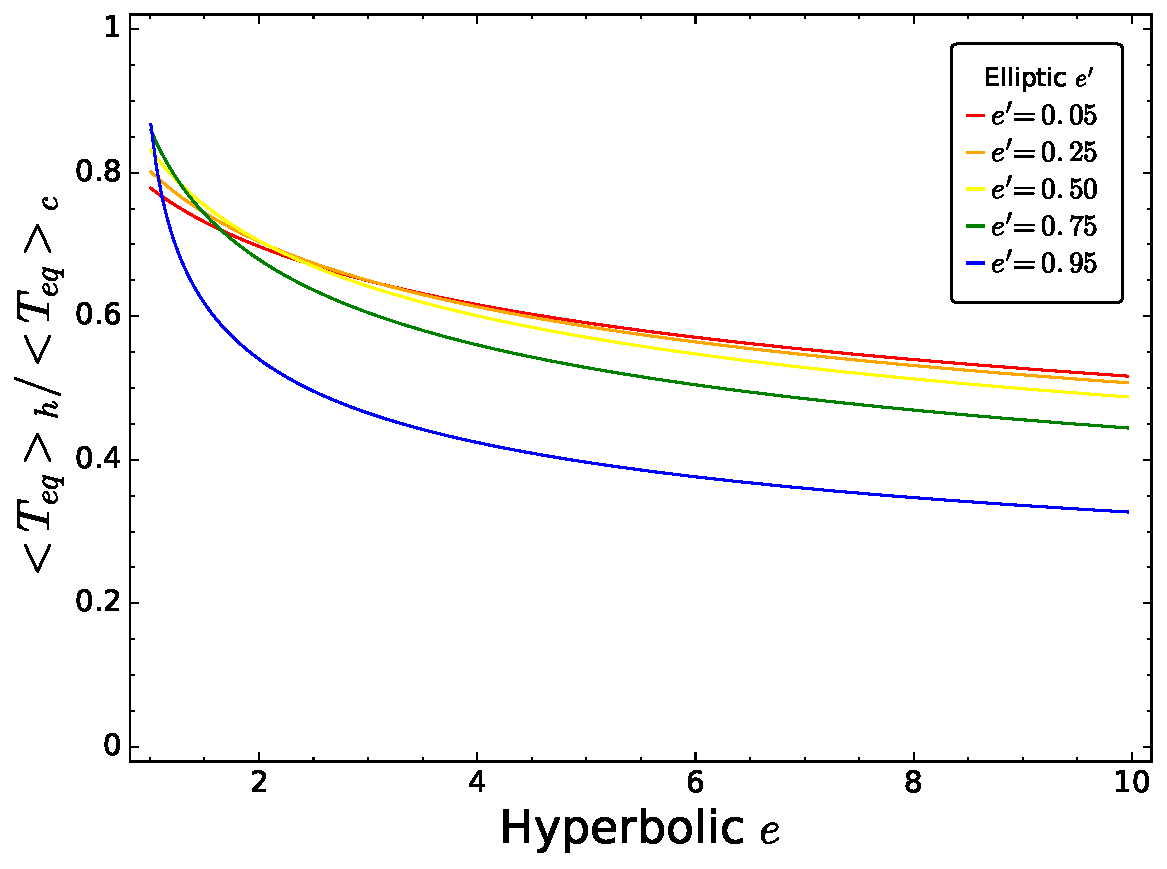
\includegraphics[width=\columnwidth]{f4.pdf}
\caption{Ratio of the average equilibrium temperature between hyperbolic trajectory and equivalent elliptic orbits with the same periastron and period (periastron time for the hyperbolic trajectory). The average temperature for hyperbolic trajectories is always less than that of an equivalent elliptic orbit.}
\label{fig4}
\end{figure}

% About how to compare al conic orbits

Probably the best way to compare the average equilibrium temperature of planetary objects in both closed or open orbits is after some critical temperature. One alternative is between the time that the surface temperatures of the object reach the sublimation temperature of a major component, such as water or carbon dioxide (Table \ref{tab:ices}). Average surface temperatures are similar to the equilibrium temperature as shown in equation \ref{eq:Ts}.

Table \ref{tab:escape} shows these properties calculated for some minor planetary bodies in escape trajectories such as 1I/'Oumuamua.

% About the albedo of 1I/'Oumuamua

In the case of 1I/'Oumuamua, it is not spherical and there is not enough photometric information over a wide range of wavelengths and phase angles to confidently calculate its bolometric albedo. However, we can just do a thermal study looking at potential $A$ values, from comet to asteroid.

% Table: Objects similar to 1I/'Oumuamua

\begin{table*}
\begin{threeparttable}
\centering
\caption{Temporal averages of orbital distance $\langle r \rangle$, stellar flux $\langle F \rangle$, and equilibrium temperature $\langle T_{eq} \rangle$ within the snow line for 'Oumuamua and some comets with similar perihelion. 1I/'Oumuamua experienced slightly higher temperatures but in a much shorter period.}
\begin{tabular}{ l c c | c c c c }
 \hline
 \hline
 & \multicolumn{2}{c}{Orbital Parameters\tnote{a}} & \multicolumn{4}{c}{Period and Temporal Averages for $T$ > 170 K\tnote{b}} \\
 \hline
 Name & $r_p$ (AU) & $e$ & $P$ (yrs) &
 	$\langle r \rangle$ (AU) & $\langle F \rangle$ & $\langle T_{eq} \rangle$ (K) \\ 
 \hline
 1I/'Oumuamua & 0.25534 & 1.19951 & 0.571 & 1.4813 & 1.70 & 261 \\
 C/1901 G1 (Great Comet) & 0.244812 & 1 & 1.01 & 1.5419 & 1.57 & 254 \\
 C/1905 X1 (Giacobini) & 0.2159002 & 1 & 1.01 & 1.5440 & 1.71 & 255 \\
C/1948 L1 (Honda-Bernasconi) & 0.207628 & 0.999875 & 0.722 & 1.5448 & 1.76 & 255 \\
 C/1975 V2 (Bradfield) & 0.21872078 & 1.00001667 & 0.725 & 1.5437 & 1.70 & 255 \\
 C/1980 Y1 (Bradfield) & 0.259823 & 0.999725 & 0.739 & 1.5413 & 1.50 & 253 \\
 C/1984 N1 (Austin) & 0.291284 & 0.999846 & 0.748 & 1.5405 & 1.38 & 252 \\
 C/1996 B2 (Hyakutake) & 0.23022931	& 0.99989867 & 0.729 & 1.5429 & 1.64 & 255 \\
 \hline
 \hline
\end{tabular}
\label{tab:escape}
	\begin{tablenotes}
	\small
\item[a]{Object elements from the NASA Solar System Dynamic website \href{https://ssd.jpl.nasa.gov/?sb$\_$elem}{https://ssd.jpl.nasa.gov/?sb$\_$elem}.}
\item[b]{Average values calculated for elliptic, parabolic and hyperbolic trajectories (equations \ref{eq:rp} to \ref{eq:Th}) and using a comet-like albedo of 0.02 for comparison purposes.}
	\end{tablenotes}
\end{threeparttable}
\end{table*}

\fix{Relevance to visiting rogue exoplanets, if any. (e.g. expected comet-like tails, atmospheric erosion. Relevance to interstellar travel. Recharge batteries from stellar flybys. Implications to panspermia.}

%% Section: Conclusion
%%%%%%%%%%%%%%%%%%%%%%%%%%%%%%%%%%%%%%%%%%%%%%%%%%

\section{Conclusion}
\label{sec:conclusion}

% About derived equations

We derived analytic expressions for the average distance, stellar flux, and equilibrium temperature of planetary bodies in hyperbolic, parabolic, and linear trajectories. Our expressions were validated with numerical solutions and applied to asteroids and comets. We found that the average equilibrium temperature of bodies in escape trajectories with constant periastron increase with eccentricity until they converge to the values for linear trajectories. We suggest that the best way to compare the thermal state between planetary bodies in elliptic and escape trajectories is within the snow line, near periastron.

% About implications to 1I/'Oumuamua

Our analysis on 1I/'Oumuamua shows that its average temperature within \fix{XXX} region was \fix{XXX} K and not high enough for a significant sublimation of any surface ices. We suggest that this low temperature and an organic crust as proposed by \citet{2017arXiv171206552F} were probably responsible for its lack of cometary activity.

%% Section: Acknowledgements
%%%%%%%%%%%%%%%%%%%%%%%%%%%%%%%%%%%%%%%%%%%%%%%%%%

\section*{Acknowledgements}

This work was supported by the Planetary Habitability Laboratory (PHL) of the University of Puerto Rico at Arecibo (UPR Arecibo). We would like to thank Guillermo Nery for helpful suggestions.

%%%%%%%%%%%%%%%%%%%%%%%%%%%%%%%%%%%%%%%%%%%%%%%%%%

%%%%%%%%%%%%%%%%%%%% REFERENCES %%%%%%%%%%%%%%%%%%

% The best way to enter references is to use BibTeX:

%\bibliographystyle{mnras}
%\bibliography{example} % if your bibtex file is called example.bib

% Alternatively you could enter them by hand, like this: This method is tedious and prone to error if you have lots of references

\begin{thebibliography}{99}

\bibitem[Bowell et al.(1989)]{1989aste.conf..524B} Bowell, E., Hapke, B., Domingue, D., et al.\ 1989, Asteroids II, 524 

\bibitem[Brown et al.(2010)]{2010AJ....139.2700B} Brown, M.~E., Ragozzine, D., Stansberry, J., \& Fraser, W.~C.\ 2010, \aj, 139, 2700 

\bibitem[Buratti et al.(2004)]{2004Icar..167..129B} Buratti, B.~J., Britt, D.~T., Soderblom, L.~A., et al.\ 2004, \icarus, 167, 129 

\bibitem[Buratti et al.(2017)]{2017Icar..287..207B} Buratti, B.~J., Hofgartner, J.~D., Hicks, M.~D., et al.\ 2017, \icarus, 287, 207 

\bibitem[Cairns \& Fuselier(2017)]{2017ApJ...834..197C} Cairns, I.~H., \& Fuselier, S.~A.\ 2017, \apj, 834, 197

\bibitem[Campins et al.(1981)]{1981motc.conf...83C} Campins, H., Gradie, J., Lebofsky, M., \& Rieke, G.\ 1981, Modern Observational Techniques for Comets,

\bibitem[Capaccioni et al.(2015)]{2015Sci...347a0628C} Capaccioni, F., Coradini, A., Filacchione, G., et al.\ 2015, Science, 347, aaa0628 

\bibitem[Cotto-Figueroa(2013)]{2013PhDT.......424C} Cotto-Figueroa, D.\ 2013, Ph.D.~Thesis,  

\bibitem[{\'C}uk(2018)]{2018ApJ...852L..15C} {\'C}uk, M.\ 2018, \apjl, 852, L15

\bibitem[de la Fuente Marcos \& de la Fuente Marcos(2017)]{2017RNAAS...1....5D} de la Fuente Marcos, C., \& de la Fuente Marcos, R.\ 2017, Research Notes of the American Astronomical Society, 1, 5

\bibitem[Delbo et al.(2015)]{2015aste.book..107D} Delbo, M., Mueller, M., Emery, J.~P., Rozitis, B., \& Capria, M.~T.\ 2015, Asteroids IV, 107 

\bibitem[Do et al.(2018)]{2018arXiv180102821D} Do, A., Tucker, M.~A., \& Tonry, J.\ 2018, arXiv:1801.02821

\bibitem[Dybczy{\'n}ski \& Kr{\'o}likowska(2017)]{2017arXiv171106618D} Dybczy{\'n}ski, P.~A., \& Kr{\'o}likowska, M.\ 2017, arXiv:1711.06618

\bibitem[Dyudina et al.(2016)]{2016ApJ...822...76D} Dyudina, U., Zhang, X., Li, L., et al.\ 2016, \apj, 822, 76 

\bibitem[Feng \& Jones(2017)]{2017arXiv171108800F} Feng, F., \& Jones, H.~R.~A.\ 2017, arXiv:1711.08800

\bibitem[Ferrin \& Zuluaga(2017)]{2017arXiv171107535F} Ferrin, I., \& Zuluaga, J.\ 2017, arXiv:1711.07535

\bibitem[Fitzsimmons et al.(2017)]{2017arXiv171206552F} Fitzsimmons, A., Snodgrass, C., Rozitis, B., et al.\ 2017, arXiv:1712.06552

\bibitem[Fraser et al.(2017)]{10.1038/s41550-018-0398-z} Fraser, W.~C., Pravec, P., Fitzsimmons, A., et al.\ 2017, Nature Astronomy, 1.

\bibitem[Fougere et al.(2016)]{2016MNRAS.462S.156F} Fougere, N., Altwegg, K., Berthelier, J.-J., et al.\ 2016, \mnras, 462, S156 

\bibitem[Gaidos et al.(2017)]{2017RNAAS...1...13G} Gaidos, E., Williams, J., \& Kraus, A.\ 2017, Research Notes of the American Astronomical Society, 1, 13

\bibitem[Gasc et al.(2017)]{2017MNRAS.469S.108G} Gasc, S., Altwegg, K., Balsiger, H., et al.\ 2017, \mnras, 469, S108 

\bibitem[Gelino et al.(1999)]{1999PCEC...24..573G} Gelino, C.~R., Marley, M., Stephens, D., Lunine, J., \& Freedman, R.\ 1999, Physics and Chemistry of the Earth C, 24, 573 

\bibitem[GSL (2016)]{GSL} GNU Scientific Library 2016, Legendre Form of Complete Elliptic Integrals. From the GNU Scientific Library. http://www.gnu.org/software/gsl

\bibitem[Hanner et al.(1981)]{1981A&A...104...42H} Hanner, M.~S., Giese, R.~H., Weiss, K., \& Zerull, R.\ 1981, \aap, 104, 42 

\bibitem[Hansen et al.(2016)]{2016MNRAS.462S.491H} Hansen, K.~C., Altwegg, K., Berthelier, J.-J., et al.\ 2016, \mnras, 462, S491 

\bibitem[Hartmann \& Cruikshank(1984)]{1984Icar...57...55H} Hartmann, W.~K., \& Cruikshank, D.~P.\ 1984, \icarus, 57, 55 

\bibitem[Hartmann et al.(1987)]{1987Icar...69...33H} Hartmann, W.~K., Tholen, D.~J., \& Cruikshank, D.~P.\ 1987, \icarus, 69, 33 

\bibitem[Johnson et al.(2015)]{2015ApJ...809...43J} Johnson, R.~E., Oza, A., Young, L.~A., Volkov, A.~N., \& Schmidt, C.\ 2015, \apj, 809, 43 

\bibitem[Jones et al.(2018)]{2018SSRv..214...20J} Jones, G.~H., Knight, M.~M., Battams, K., et al.\ 2018, \ssr, 214, \#20 

\bibitem[Kennedy \& Kenyon(2008)]{2008ApJ...673..502K} Kennedy, G.~M., \& Kenyon, S.~J.\ 2008, \apj, 673, 502-512 

\bibitem[Knight et al.(2017)]{2017ApJ...851L..31K} Knight, M.~M., Protopapa, S., Kelley, M.~S.~P., et al.\ 2017, \apjl, 851, L31 

\bibitem[Lamy et al.(2004)]{2004come.book..223L} Lamy, P.~L., Toth, I., Fernandez, Y.~R., \& Weaver, H.~A.\ 2004, Comets II, 223 

\bibitem[Li et al.(2013)]{2013Icar..226.1252L} Li, J.-Y., Le Corre, L., Schr{\"o}der, S.~E., et al.\ 2013, \icarus, 226, 1252 

\bibitem[Mallama(2017)]{2017arXiv170302670M} Mallama, A.\ 2017, arXiv:1703.02670 

\bibitem[Mamajek(2017)]{2017RNAAS...1...21M} Mamajek, E.\ 2017, Research Notes of the American Astronomical Society, 1, 21 

\bibitem[Mayorga et al.(2016)]{2016AJ....152..209M} Mayorga, L.~C., Jackiewicz, J., Rages, K., et al.\ 2016, \aj, 152, 209 

\bibitem[Meech et al.(2017a)]{2017MPEC....U..183M} Meech, K., Bacci, P., Maestripieri, M., et al.\ 2017, Minor Planet Electronic Circulars, 2017-U183

\bibitem[Meech et al.(2017b)] {2017NatureMeech} Meech K. J., et al., 2017, \nat, 552, 378

\bibitem[M{\'e}ndez \& Rivera-Valent{\'{\i}}n(2017)]{2017ApJ...837L...1M} M{\'e}ndez, A., \& Rivera-Valent{\'{\i}}n, E.~G.\ 2017, \apjl, 837, L1 

\bibitem[Mumma \& Charnley(2011)]{2011ARA&A..49..471M} Mumma, M.~J., \& Charnley, S.~B.\ 2011, \araa, 49, 471 

\bibitem[NASA/JPL SSD(2018)]{SSD(2018)} NASA/JPL Solar System Dynamics. https://ssd.jpl.nasa.gov/

\bibitem[Nugent et al.(2015)]{2015ApJ...814..117N} Nugent, C.~R., Mainzer, A., Masiero, J., et al.\ 2015, \apj, 814, 117 

\bibitem[P{\'a}l et al.(2012)]{2012A&A...541L...6P} P{\'a}l, A., Kiss, C., M{\"u}ller, T.~G., et al.\ 2012, \aap, 541, L6 

\bibitem[P{\'a}l et al.(2016)]{2016AJ....151..117P} P{\'a}l, A., Kiss, C., M{\"u}ller, T.~G., et al.\ 2016, \aj, 151, 117 

\bibitem[Portegies Zwart et al.(2017)]{2017arXiv171103558P} Portegies Zwart, S., Pelupessy, I., Bedorf, J., Cai, M., \& Torres, S.\ 2017, arXiv:1711.03558

\bibitem[Russell(1916)]{1916PNAS....2...74R} Russell, H.~N.\ 1916, Proceedings of the National Academy of Science, 2, 74 

\bibitem[Sicardy et al.(2011)]{2011Natur.478..493S} Sicardy, B., Ortiz, J.~L., Assafin, M., et al.\ 2011, \nat, 478, 493 

\bibitem[Schl{\"a}ppi et al.(2008)]{2008Icar..195..674S} Schl{\"a}ppi, B., Altwegg, K., \& Wurz, P.\ 2008, \icarus, 195, 674 

\bibitem[Schneider(2017)]{2017RNAAS...1...18S} Schneider, J.\ 2017, Research Notes of the American Astronomical Society, 1, 18

\bibitem[Schorghofer(2008)]{2008ApJ...682..697S} Schorghofer, N.\ 2008, \apj, 682, 697-705 

\bibitem[Schorghofer(2016)]{2016Icar..276...88S} Schorghofer, N.\ 2016, \icarus, 276, 88

\bibitem[Sch{\"o}rghofer \& Hsieh(2018)]{2018arXiv180201293S} Sch{\"o}rghofer, N., \& Hsieh, H.~H.\ 2018, arXiv:1802.01293

\bibitem[Shestopalov \& Golubeva(2011)]{2011LPI....42.1028S} Shestopalov, D.~I., \& Golubeva, L.~F.\ 2011, Lunar and Planetary Science Conference, 42, 1028

\bibitem[Takir et al.(2015)]{2015Icar..252..393T} Takir, D., Clark, B.~E., Drouet d'Aubigny, C., et al.\ 2015, \icarus, 252, 393 

\bibitem[Usui et al.(2013)]{2013ApJ...762...56U} Usui, F., Kasuga, T., Hasegawa, S., et al.\ 2013, \apj, 762, 56 

\bibitem[Weissman \& Kieffer(1981)]{1981Icar...47..302W} Weissman, P.~R., \& Kieffer, H.~H.\ 1981, \icarus, 47, 302 

\bibitem[Weisstein (2016)]{MathWorld} Weisstein, Eric W. 2016, Complete Elliptic Integral of the Second Kind. From MathWorld--A Wolfram Web Resource. http://mathworld.wolfram.com

\bibitem[Wright(2017)]{2017RNAAS...1...38W} Wright, J.~T.\ 2017, Research Notes of the American Astronomical Society, 1, 38 

\bibitem[Zhang(2018)]{2018ApJ...852L..13Z} Zhang, Q.\ 2018, \apjl, 852, L13

\bibitem[Zuluaga et al.(2017)]{2017arXiv171109397Z} Zuluaga, J.~I., Sanchez-Hernandez, O., Sucerquia, M., \& Ferrin, I.\ 2017, arXiv:1711.09397

\end{thebibliography}

%%%%%%%%%%%%%%%%%%%%%%%%%%%%%%%%%%%%%%%%%%%%%%%%%%

%%%%%%%%%%%%%%%%% APPENDICES %%%%%%%%%%%%%%%%%%%%%

\appendix
\section{Orbital Elements}
\label{sec:elements}

% Table: Orbital elements summary

% \begin{landscape}
\begin{table*}
\begin{threeparttable}
% \centering
\caption{Orbital elements of circular, elliptic, parabolic, hyperbolic, and linear trajectories. Only the linear trajectory is an impossible path.}
\begin{tabular}{l c c c c c}
\hline \hline
Orbital Element & Circular & Elliptic & Parabolic &
 	Hyperbolic\tnote{a} & Linear \\
& $e=0$ & $0<e<1$ & $e=1$ & $1<e<\infty$ & $e=\infty$ \\
 \hline
 Position, $r(f)$ & $r=a$ & $r=\frac{a(1-e^2)}{1+e\cos{f}}$ & $r=r_p\frac{2}{1+cos{f}}$ & $r=r_p\frac{1+e}{1+e\cos{f}}$  & $r=r_p\csc{f}$ \\
 Position, $r(E, D,$ or $H)$ & $r=a$ & $r=a(1-e\cos{E})$ & $r=r_p(1+D^2)$ & $r=r_p\frac{e\cosh{H}-1}{e-1}$  & $r=r_p\cosh{H}$ \\
 Periastron, $r_p$ & $r_p=a$ & $r_p=a(1-e)$ & $r_p=r_p$ & $r_p=r_p$ & $r_p=r_p$ \\
 Apastron, $r_a$ & $r_a=a$ & $r_a=a(1+e)$ & $r_a=\infty$ & $r_a=\infty$ & $r_a=\infty$ \\
 True Anomaly, $f$ & $f=E$ & $\tan{\frac{f}{2}}=\sqrt{\frac{e+1}{e-1}}\tan{\frac{E}{2}}$ & $\tan{\frac{f}{2}}=D$ & $\tan{\frac{f}{2}}=\sqrt{\frac{e+1}{e-1}}\tanh{\frac{H}{2}}$ & $\tan{\frac{f}{2}}=\tanh{\frac{H}{2}}$ \\
 Conic Anomaly, $E, D, or H$ & $E=f$ & $\cos{E}=\frac{e+\cos{f}}{1+e\cos{f}}$ & $D=\tan{\frac{f}{2}}$ & $\tanh{\frac{H}{2}}=\sqrt{\frac{e-1}{e+1}}\tan{\frac{f}{2}}$ & $\tanh{\frac{H}{2}}=\tan{\frac{f}{2}}$ \\
 Mean Anomaly, $M$ & $M=E$ & $M=E-e\sin{E}$ & $M=D+\frac{1}{3}D^3$ & $M=e\sinh{H}-H$ & undefined \\
 Time from Periastron, $t$ & $t=M\sqrt{\frac{a^3}{\mu}} + t_o$ & $t=M\sqrt{\frac{a^3}{\mu}} + t_o$ & $t=M\sqrt{\frac{2r_p^3}{\mu}} + t_o$ & $t=M\sqrt{\frac{r_p^3}{\mu(e-1)^3}} + t_o$ & undefined \\
 Period, $P$ & $P=2\pi\sqrt{\frac{a^3}{\mu}}$ & $P=2\pi\sqrt{\frac{a^3}{\mu}}$ & $P=2M_o\sqrt{\frac{2r_p^3}{\mu}}$ & $P=2M_o\sqrt{\frac{r_p^3}{\mu(e-1)^3}}$ & undefined \\
 True Anomaly Range & $0\leq f \leq 2\pi$ & $0\leq f \leq 2\pi$ & $-\pi< f < +\pi$ & $-\cos^{-1}{(-\frac{1}{e})} < f < +\cos^{-1}{(-\frac{1}{e})}$ & $-\frac{\pi}{2} < f < +\frac{\pi}{2}$ \\
 Conic Anomaly Range & $0\leq E \leq 2\pi$ & $0\leq E \leq 2\pi$ & $-\infty < D < +\infty$ & $-\infty< H < +\infty$ & $-\infty< H < +\infty$ \\
 Mean Anomaly Range & $0\leq M \leq 2\pi$ & $0\leq M \leq 2\pi$ & $-\infty< M < +\infty$ & $-\infty < M < +\infty$ & undefined \\
 \hline
 \hline
\end{tabular}
\label{tab:summary}
	\begin{tablenotes}
	\small
\item[a]{Hyperbolic equations are expressed in terms of the periastron instead of semi-major axis.}
	\end{tablenotes}
\end{threeparttable}
\end{table*}
% \end{landscape}

%%%%%%%%%%%%%%%%%%%%%%%%%%%%%%%%%%%%%%%%%%%%%%%%%%

% Don't change these lines

\bsp	% typesetting comment
\label{lastpage}
\end{document}

% End of mnras_template.tex